%!TEX root = ../report.tex

\section{Experiments}
\subsection{Simulated examples}
In this next section we present the results and intuition behind the first three experiments in \cite{sghmc}. We reproduced these three experiments by converting the MATLAB codes provided by the authors \citeauthor{sghmc} \cite{simu_code} into Python code. We used this, rather than our own implementation of SGHMC, as our version does not directly interface with a given potential function, but only Pyro PPs. The experiments that we replicated mostly consisted of checking whether the samples produced by SGHMC and the other algorithms actually follow the target distribution.

\subsubsection*{Experiment 1}
As in \cite{sghmc} we considered the potential function $U(\theta) = -2\theta^2 + \theta^4$. This is sufficient for the purpose of checking the convergence to the target distribution for HMC. To check that the theoretical convergence of Naïve SGHMC and SGHMC are true or not we introduce noise into the gradient, and so we set:
$$\nabla \widetilde{U}(\theta) = \nabla U(\theta) + \mathcal{N}(0,4)$$
This now corresponds to setting the noise covariance to $V=4$ in the description of Naïve SGHMC we gave earlier. We then take samples using HMC, Naïve SGHMC and SGHMC. We also note that both HMC and Naïve SGHMC use Metropolis Hastings corrections (MH), while SGHMC has no need to. This allows us to test 5 algorithms: HMC (with MH), HMC (without MH), Naïve SGHMC (with MH), Naïve SGHMC (without MH), and SGHMC. As a small extension we also performed the same experiment with the potential function $U(\theta) = \theta^2$. The results are shown in \cref{fig:demo1,fig:demo2}.
\begin{figure}[h!]
  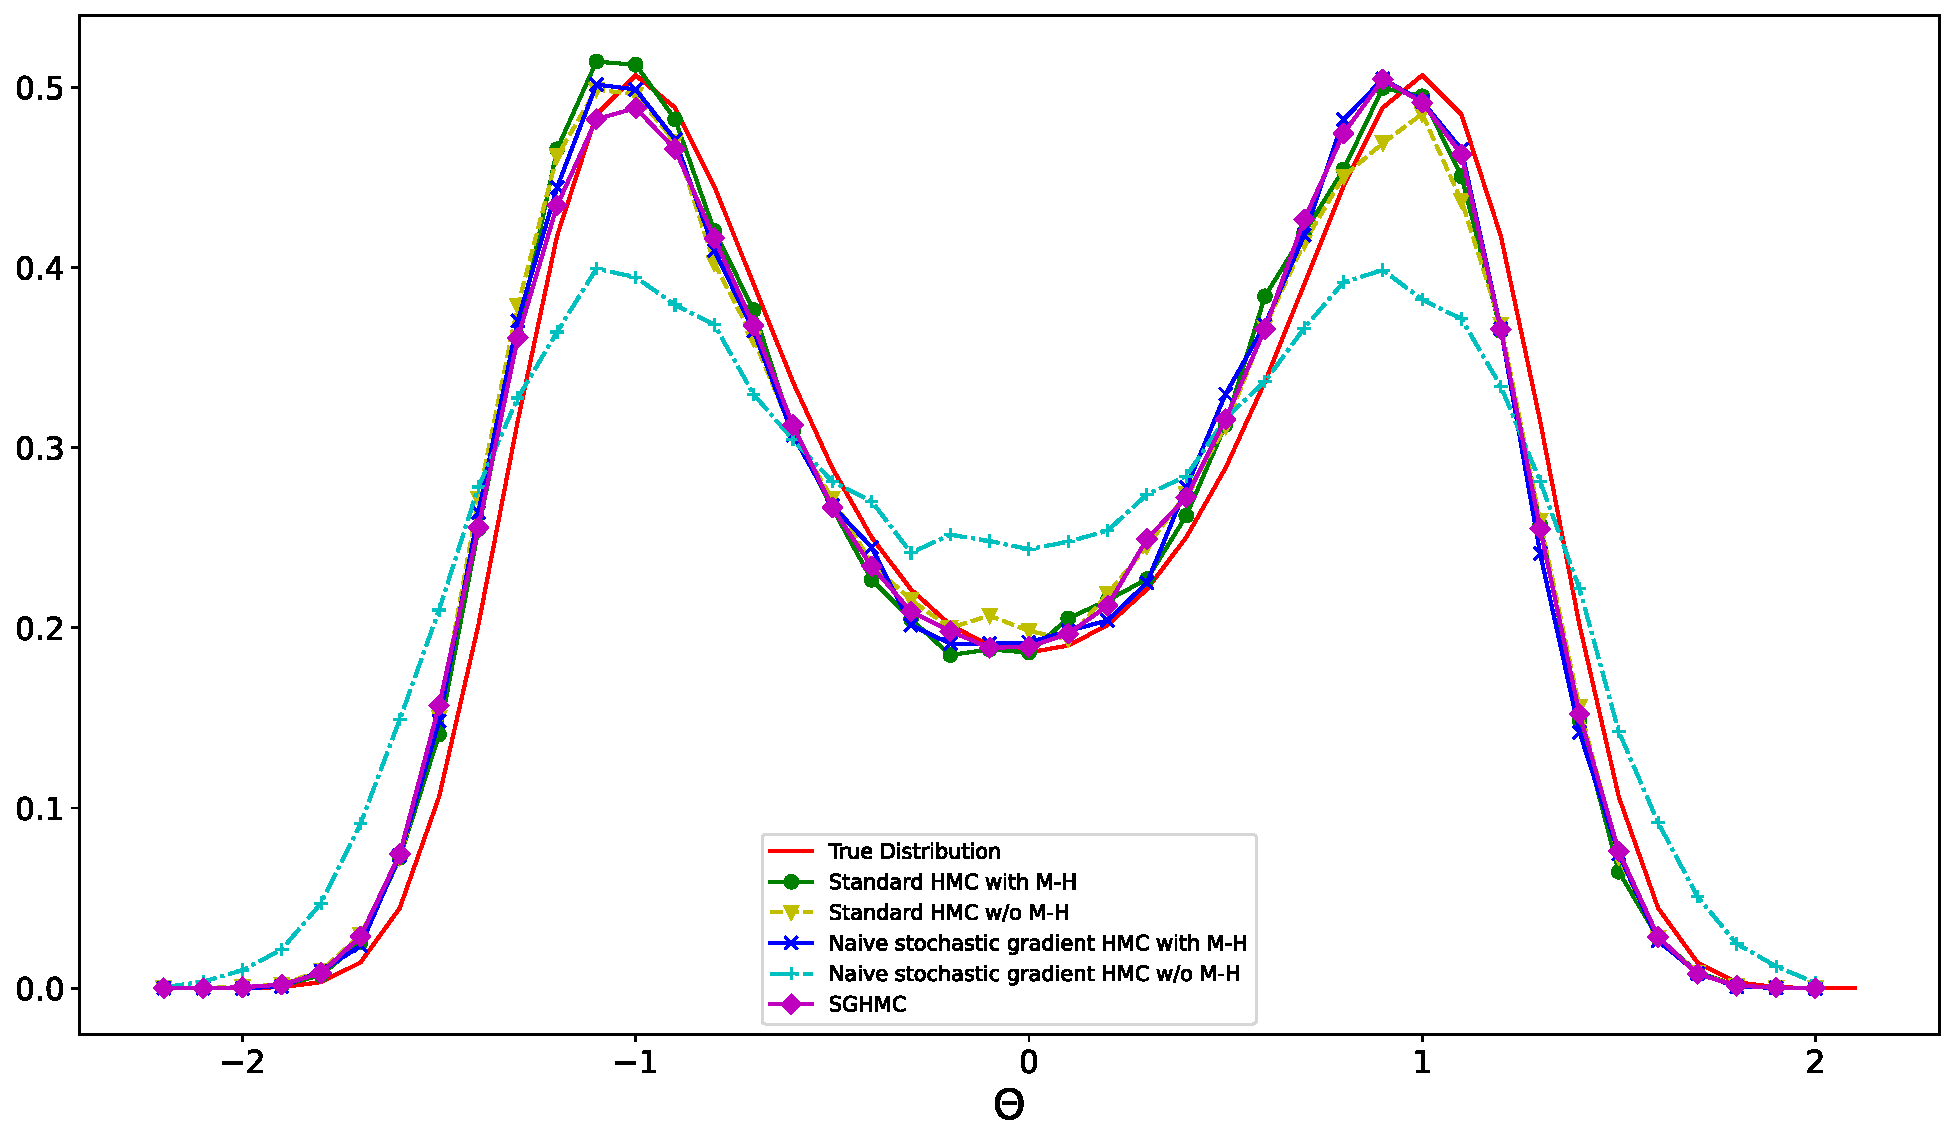
\includegraphics[width=.9\linewidth]{parts/Images/fig1a.pdf}
  \caption{Distributions of different sampling algorithms for the target function $U(\theta) = -2\theta^2 + \theta^4$}
  \label{fig1a}
  \label{fig:demo1}
\end{figure}
\begin{figure}[h!]
  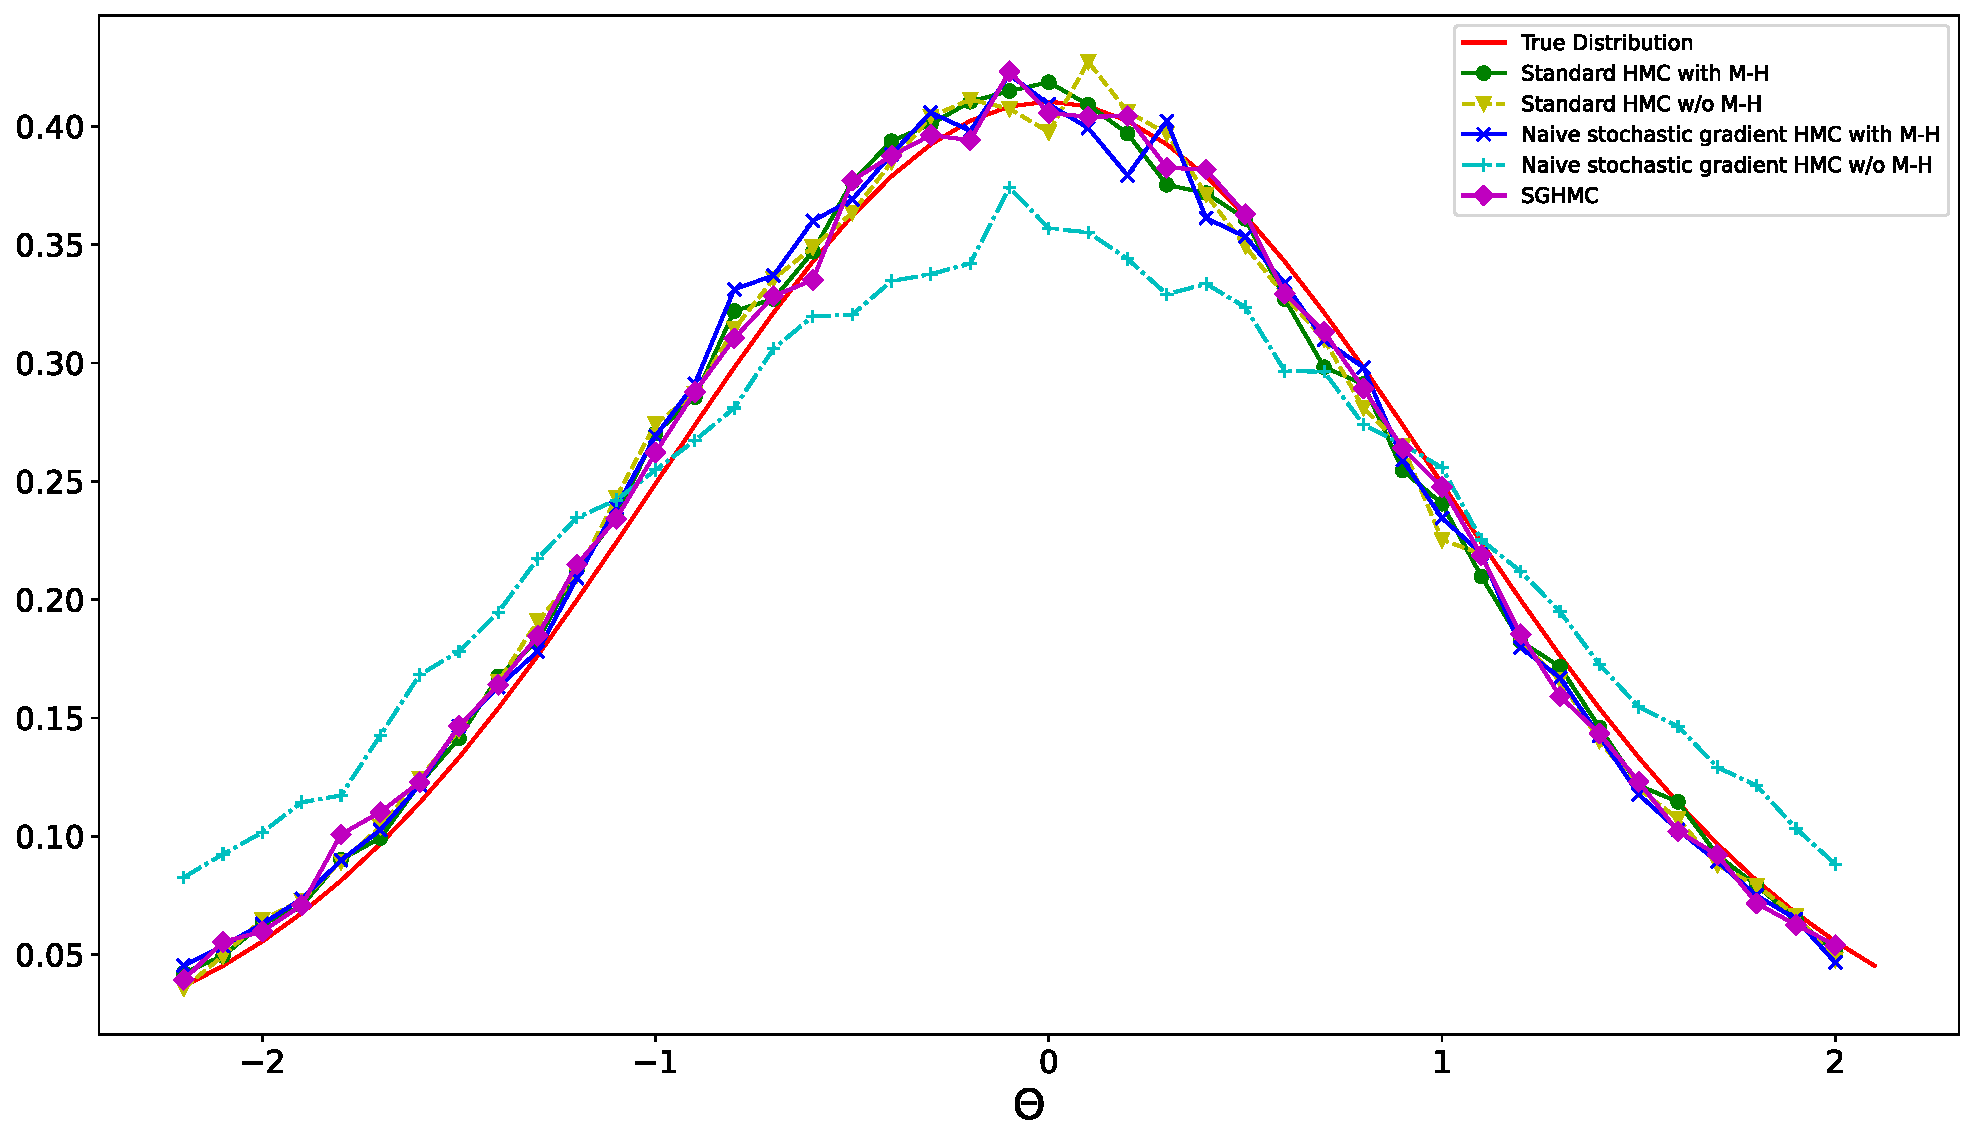
\includegraphics[width=.9\linewidth]{parts/Images/fig1b.pdf}
  \caption{Distributions of different sampling algorithms for the target function $U(\theta) = \frac{1}{2}\theta^2$}
  \label{fig:demo2}
\end{figure}
It can be seen that both HMC algorithms perform well, as does Naïve SGHMC with MH corrections. However, as we already discussed these two algorithms are computationally demanding when used on large datasets. Furthermore, Naïve SGHMC does not converge to the correct distribution, empirically confirming Corollary 3.1 in \cite{sghmc}. On the other hand, SGHMC is fast and maintains the target distribution as its invariant distribution and so can be considered as a useful candidate for scalable Bayesian inference. We note here that our diagram for $U(\theta) = -2\theta^2 + \theta^4$ mirrors Figure 1 the paper very closely.
\subsubsection*{Experiment 2}
Next we used HMC to sample $(\theta, r)$ from the potential function $U(\theta) = \frac{1}{2}\theta^2$ , and as before, we simulated noisy gradient as follows: $\nabla \widetilde{U}(\theta) = \nabla U(\theta) + \mathcal{N}(0,4)$. Except in the case specified, we did not resample the momentum $r$ here. We plotted the samples found using perfect gradient Hamiltonian dynamics (HMC), noisy gradient Hamiltonian dynamics (effectively Naïve SGHMC), noisy gradient Hamiltonian dynamics with momentum resampling and noisy Hamiltonian dynamics with friction (effectively SGHMC). We present the results below in \cref{fig:theta_r_samples}, which closely match those of \cite{sghmc}. Note that in \cite{sghmc} the \citeauthor{sghmc} claimed that the samplers were run for 15000 steps, however their plot shows far fewer points. We simulated the aforementioned algorithms for 15000 steps and for 360, and decided that the later better illustrated the dynamics and aligned more closely with the original plot.
\begin{figure}[h!]
    \centering
    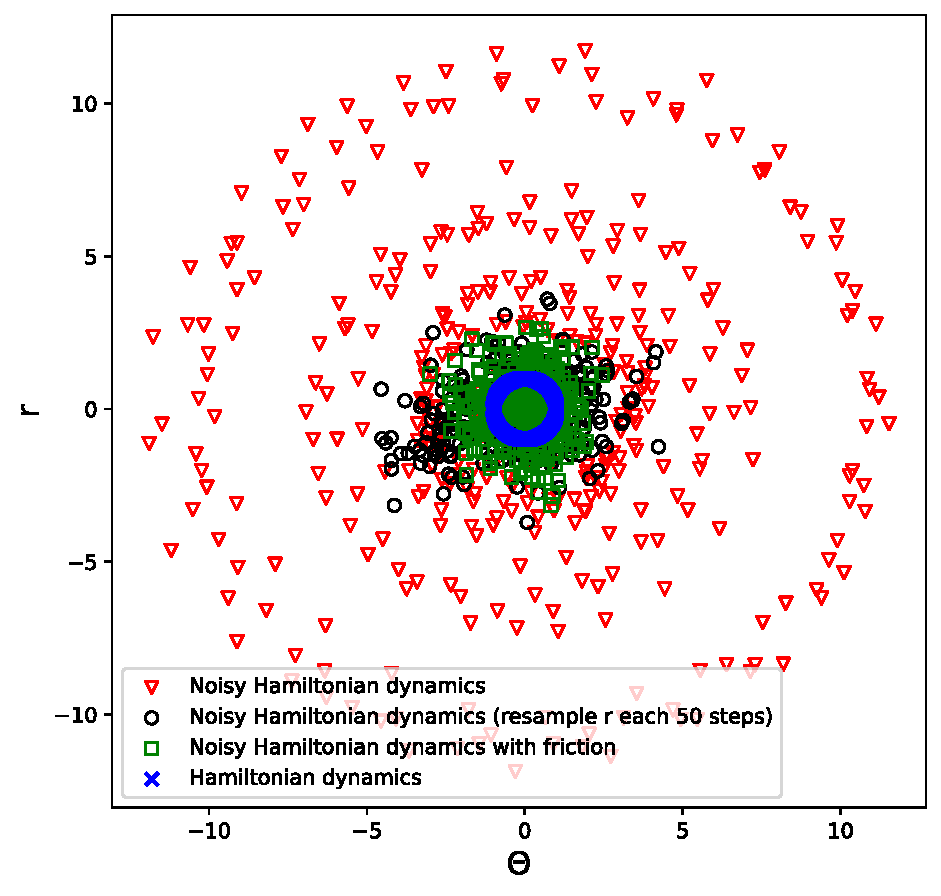
\includegraphics[width=0.9\linewidth]{parts/Images/fig2a.pdf}%
    \caption{Plotting the trajectory of $(\theta, r)$ under various samplers for 360 steps}
     \label{fig:theta_r_samples}%
\end{figure}
These results show that friction (green) keeps Hamiltonian dynamics much closer to the true Hamiltonian dynamics (blue) in a noisy system. Resampling the momentum every 50 steps also seems to mitigate the problem which is probably why the authors \citeauthor{sghmc} include it in their pseudocode description of SGHMC. \cref{fig:theta_r_samples} also supports the results of Theorem 3.1 in \cite{sghmc}, that the sampled distribution tends to the uniform distribution over time, rather than the target distribution.
\subsubsection*{Experiment 3}
Finally, we consider the following correlated distribution, as is done in \cite{sghmc}. \citeauthor{sghmc} note that the strength of HMC is typically in its efficiency in sampling from correlated distributions, and that SGHMC maintains this property. We reproduced the following experiment in \cite{sghmc}, where the authors \citeauthor{sghmc} compare the autocorrelation times of SGHMC and SGLD by considering the following potential function: $U(\theta)=\frac{1}{2}\theta^T\Sigma^{-1}\theta$, with $\nabla \widetilde{U}(\theta) = \Sigma^{-1}\theta + \mathcal{N}(0,I)$, where $\Sigma_{11} = \Sigma_{22} = 1$ and $\rho = \Sigma_{12} = 0.9$.  

\cref{fig:sghmc vs sgld} presents the results of this experiment. The first plot shows 50 samples produced using both algorithms. The second shows the average absolute error of the sample covariance against autocorrelation time (for more details see \cite{sghmc}.
\begin{figure}[h!]
  \begin{subfigure}{.5\textwidth}
  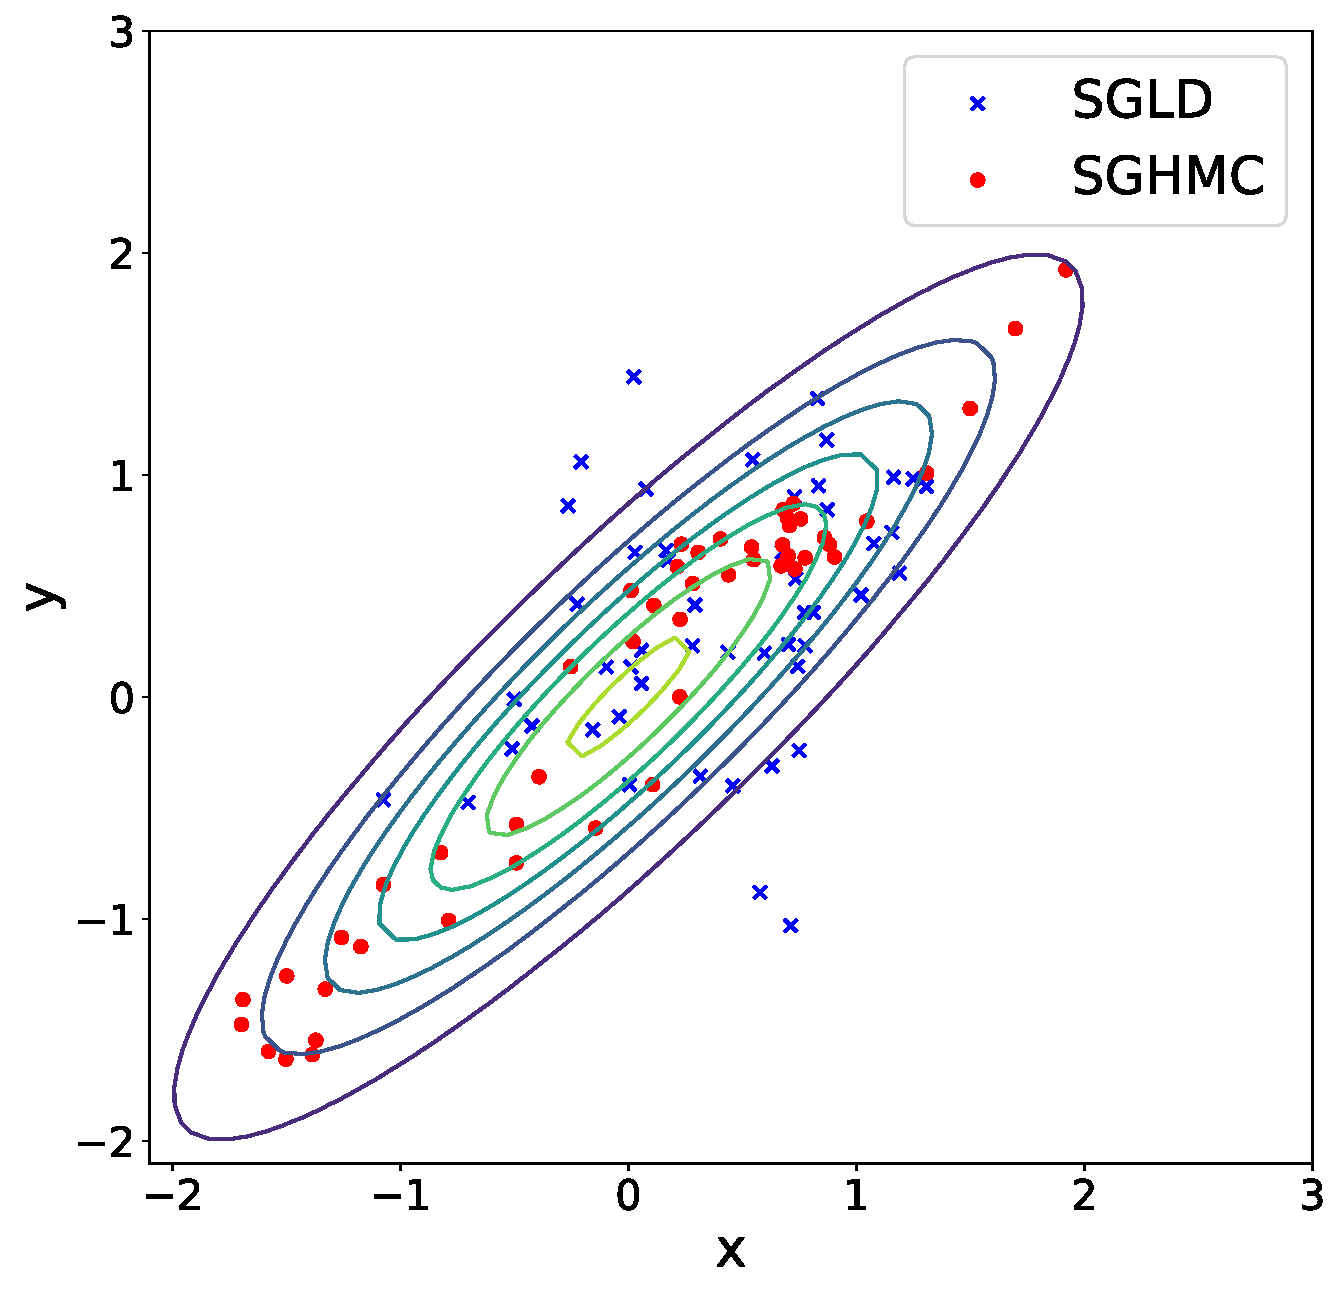
\includegraphics[width=.95\linewidth]{parts/Images/fig3b.pdf}
  \caption{First 50 samples of SGHMC and SGLD}
  \end{subfigure}
  \begin{subfigure}{.5\textwidth}
  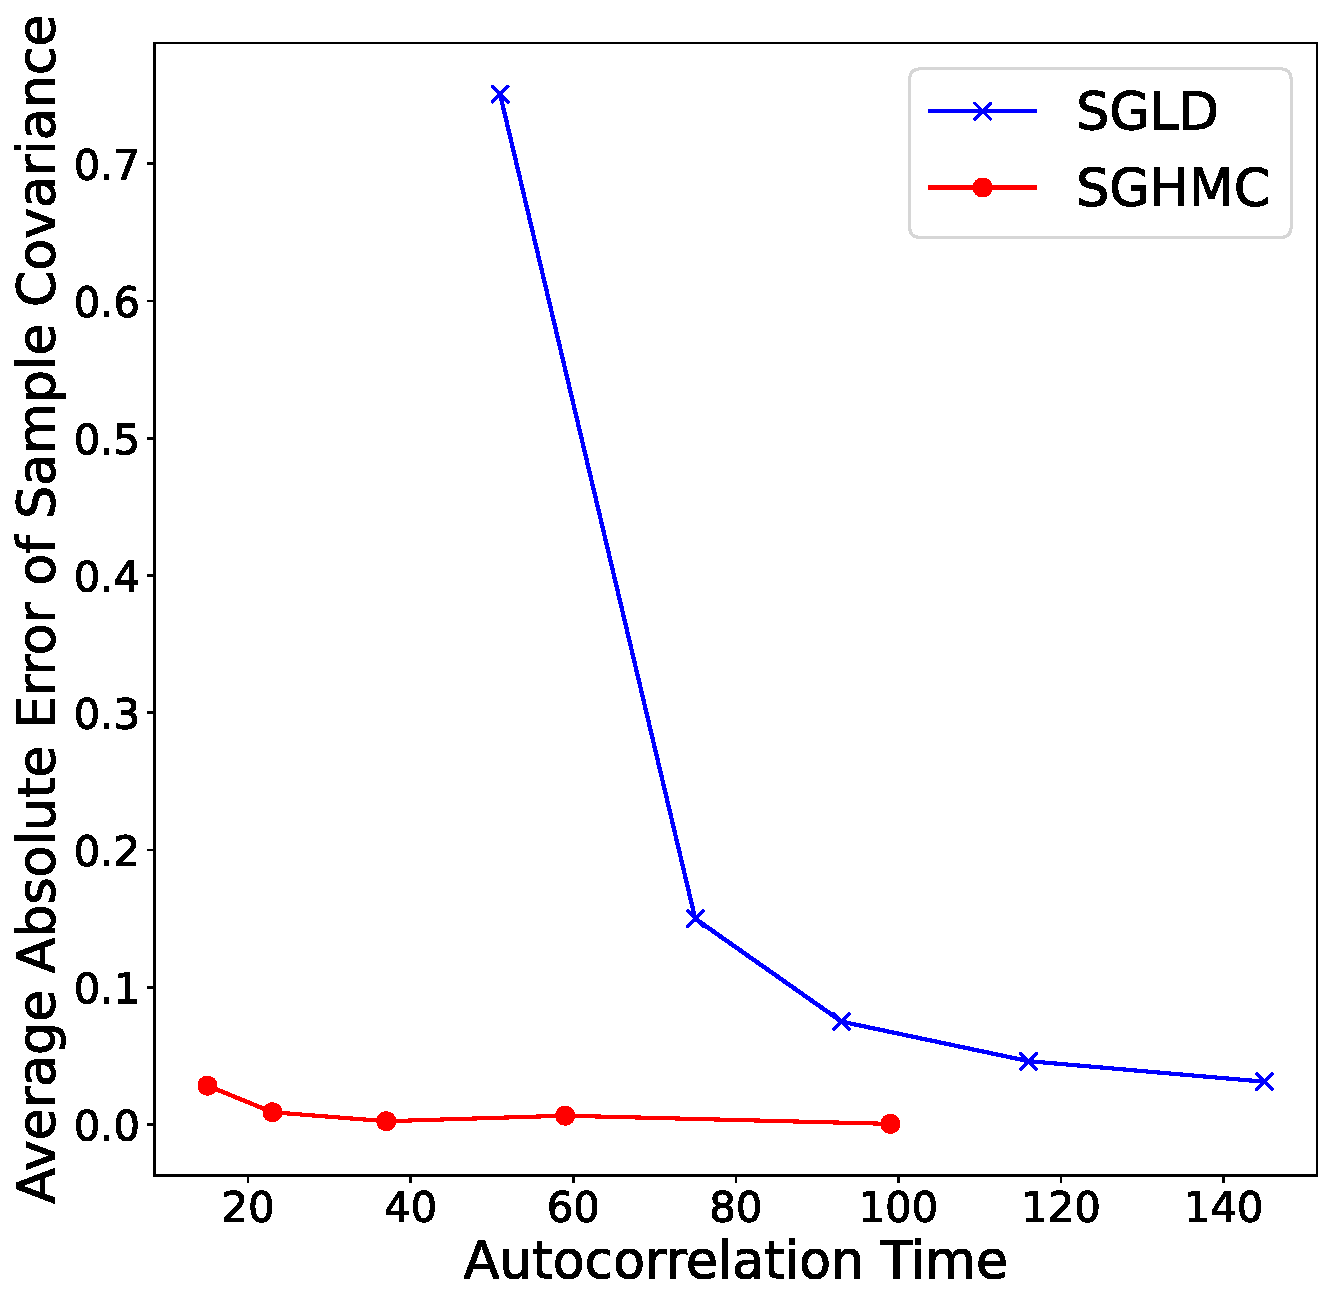
\includegraphics[width=.95\linewidth]{parts/Images/fig3a.pdf}
  \caption{Autocorrelation time versus estimation error for the five setting}
  \end{subfigure}%
  \caption{Contrasting sampling of a bivariate Gaussian with correlation using SGHMC versus SGLD.}
  \label{fig:sghmc vs sgld}
\end{figure}
We see that SGHMC samples quickly becomec uncorrelated, which is not the case for the SGLD samples - this indicates that there is an advantage in adopting SGHMC. While both SGHMC and SGLD accurately sample from the posterior, SGHMC needs fewer samples to fully explore the posterior distribution and we see that after just a few samples SGHMC has already explored the tails of the target distribution. Therefore we empirically see that SGHMC has a much faster mixing time than SGLD which is an inherent advantage.

\subsection{Bayesian Neural Networks for Classification}
For the Bayesian neural network (BNN) MNIST classification we actually used the reparameterisation of SGHMC described in the section ``Connection to SGD with Momentum'' of \cite{sghmc}. The SGHMC algorithm is reframed in terms of learning rate and momentum decay, and simulates the following dynamics instead:
$$\begin{cases}
\delta \theta = v\\
\delta v = - \eta \nabla \wt{U}(\theta) - \alpha v + \mathcal{N}(0, 2(\alpha - \wh{\beta}) \eta)
\end{cases}
$$
where $\eta = \epsilon^2 M^{-1}, \alpha = \epsilon M^{-1}C, \wh{\beta} = \eta M^{-1}\wh{B}$. In all our experiments in this section we set the mass matrix $M $ to the identity, and the noise model $\wh{\beta} = \wh{B} = 0$. Other than the architecture of the BNN there are now only 3 hyperparameters for SGHMC, the learning rate $\eta$, the momentum decay $\alpha$ and the batch size $|\wt{\D}|$, in all our experiments we fixed $|\wt{\D}| = 500$ which follows from \cite{sghmc}.

To build on top of the work in \cite{sghmc} we implemented learning rate annealing for SGLD, and following \cite{sgld} we weighted the samples by the learning rate as follows:
$$\mathbf{\hat p} := \frac{\sum^T_{t=1} \eta_t f_{\theta_t}(\textbf{x})}{\sum^T_{t=1} \eta_t}$$
Where $f_\theta$ is our classifier parameterized by $\theta$, $\mathbf{x}$ can be thought of as the ``test set" and $\mathbf{\hat p}$ is an unormalized probability vector. Note that since $f$ is a classifier we can ignore the denominator because it won't affect the argmax. Our BNN followed the same architecture as in \cite{sghmc}, that is one linear layer with 100 hidden units followed by ReLU activation followed by another linear layer and a log softmax for multi-class classification. The weights and biases for both linear layers are sampled from univariate standard normal distributions, but the Pyro method \texttt{to\_event()} declares dependence between the parameters. 

Our implementations of SGD and SGD with momentum are meant to be used directly with Pyro, and so Gaussian priors on the weights and biases is equivalent to L2 regularization in the non-Bayesian paradigm. We experimented with regularization strengths of $\lambda \in \{0.1, 1.0, 10.0\}$ and found $\lambda = 1.0$ to be the most effective. Additionally we implemented weight decay for both SGD and SGD with momentum but found that this didn't improve anything in this setting.

For the momentum based algorithms, SGHMC and SGD with momentum, we tried $\eta \in \{1.0, 2.0, 4.0, 8.0 \} \times 10^{-6}$, and $\alpha \in \{0.1, 0.01, 0.001 \}$. For SGHMC the best configuration was $\eta = 2.0\times 10^{-6}, \alpha=0.01$, and for SGD with momentum the best configuration was $\eta = 1.0\times 10^{-6}, \alpha=0.01$.

For SGLD and SGD, we tried $\eta \in \{1.0, 2.0, 4.0, 6.0\} \times 10^{-5}$, for SGLD we also tried learning rate annealing but it proved not to make much of a difference in this setting so we ignored it in the end. The best configuration for SGLD was $\eta = 4.0\times 10^{-5}$, and for SGD the best configuration was $\eta = 1.0\times 10^{-5}$.

For MNIST we ran each of the algorithms for 800 epochs with 50 warmup epochs. For the sampling algorithms the idea is that after warmup we have reached the posterior; we then perform Bayesian averaging over the entire set $\Theta$, which consists of all of the sampled parameterizations of the BNN up to that point. The general framework of Bayesian averaging in classification tasks is described in Section II of \cite{hands-on-bnn} and is used to report the test error as follows:
$$\mathbf{\hat p} := \sum_{\theta_i \in \Theta} f_{\theta_i} (\mathbf{x}) \qquad ; \qquad \mathbf{\hat y} = \text{argmax}_{i} \{ p_i \in \mathbf{\hat p} \}$$
However, for the optimization algorithms we take just the most recent sample / set of parameters as a point estimate and report the test error.  \cref{fig:MNIST} presents our results.
\begin{figure}[h!]
\centering
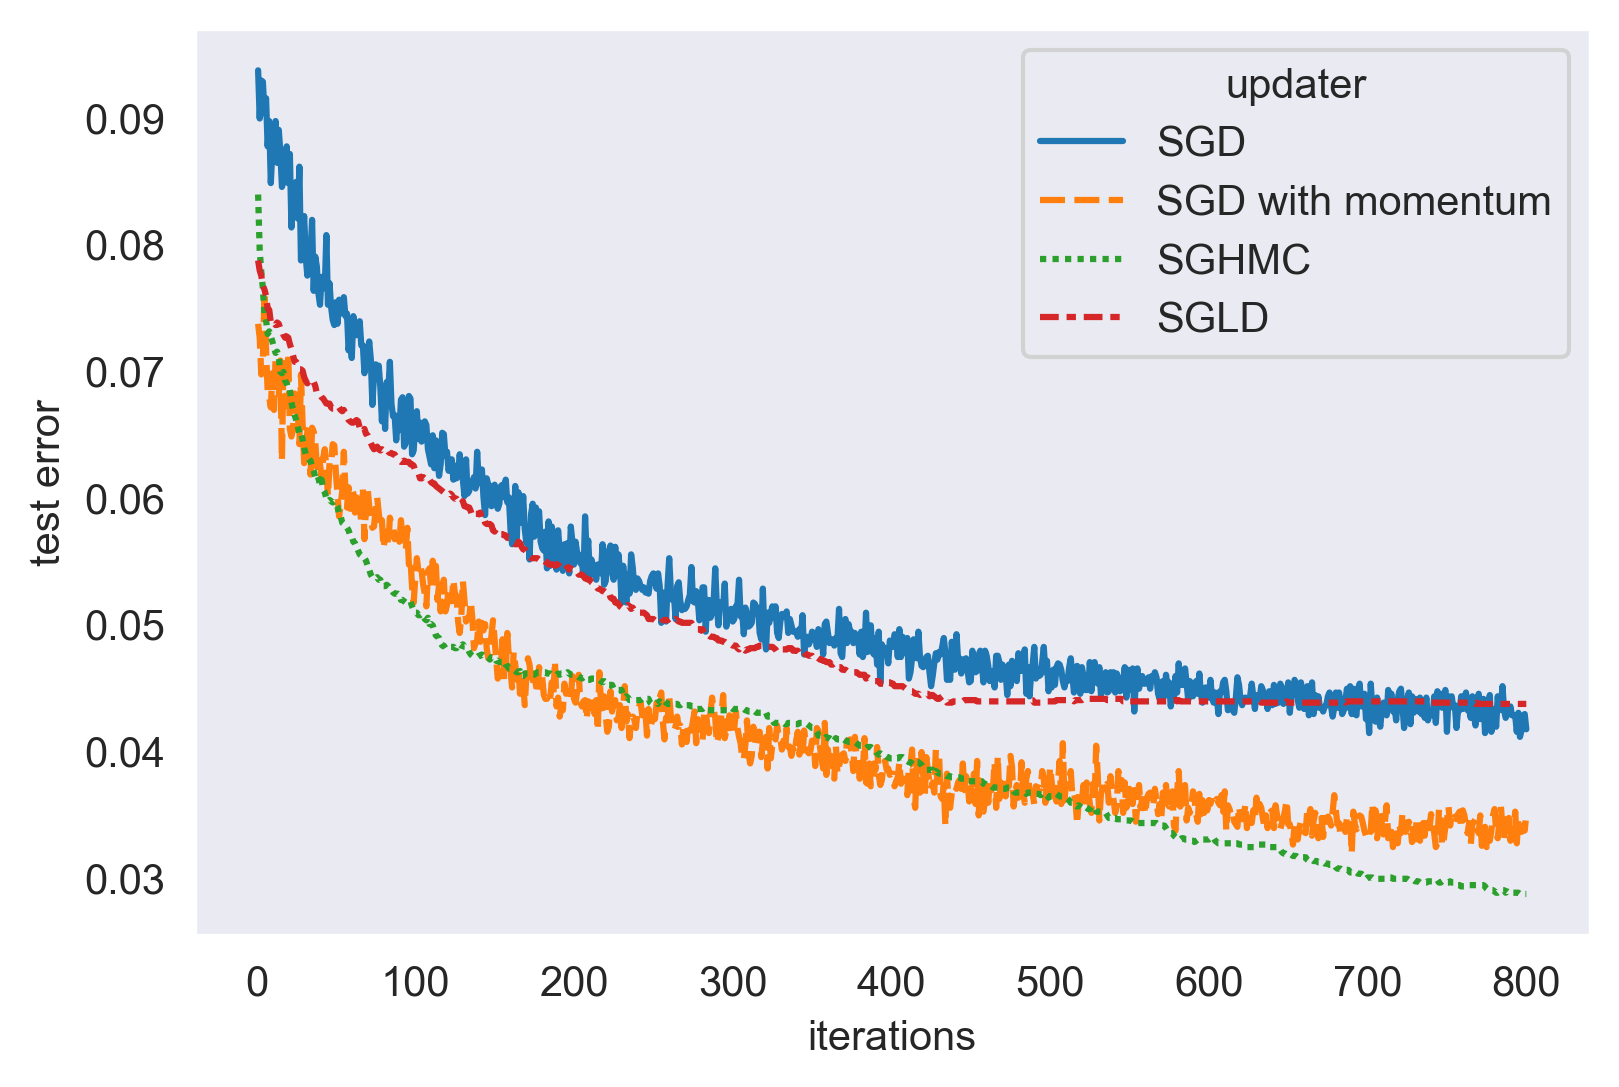
\includegraphics[width=100mm]{parts/Images/MNIST.png}
\caption{Reproducing the MNIST classification experiment from \cite{sghmc}; SGHMC ($\eta = 2.0\times 10^{-6}, \alpha=0.01, \texttt{resample\_n} =0$ ), SGLD ($\eta = 4.0\times 10^{-5}$), SGD ($\eta = 1.0\times 10^{-5}$), SGD with momentum ($\eta = 1.0\times 10^{-6}, \alpha=0.01$)}
\label{fig:MNIST}
\end{figure}
The results we get from MNIST classification align very closely with those in \cite{sghmc} and so we come to the same conclusion; the need for scalable and efficient Bayesian inference algorithms. The key benefit of BNNs is that we are not overconfident on out-of-distribution examples, \cref{fig:B} illustrates that we still maintain this property when using SGHMC to approximately sample from the posterior distribution. We additionally conducted a brief comparison between Variational Inference (VI) and SGHMC in this setting, \cref{fig:VI} outlines our findings.
\begin{figure}[h!]
\centering
\begin{subfigure}{.5\textwidth}
  \centering
  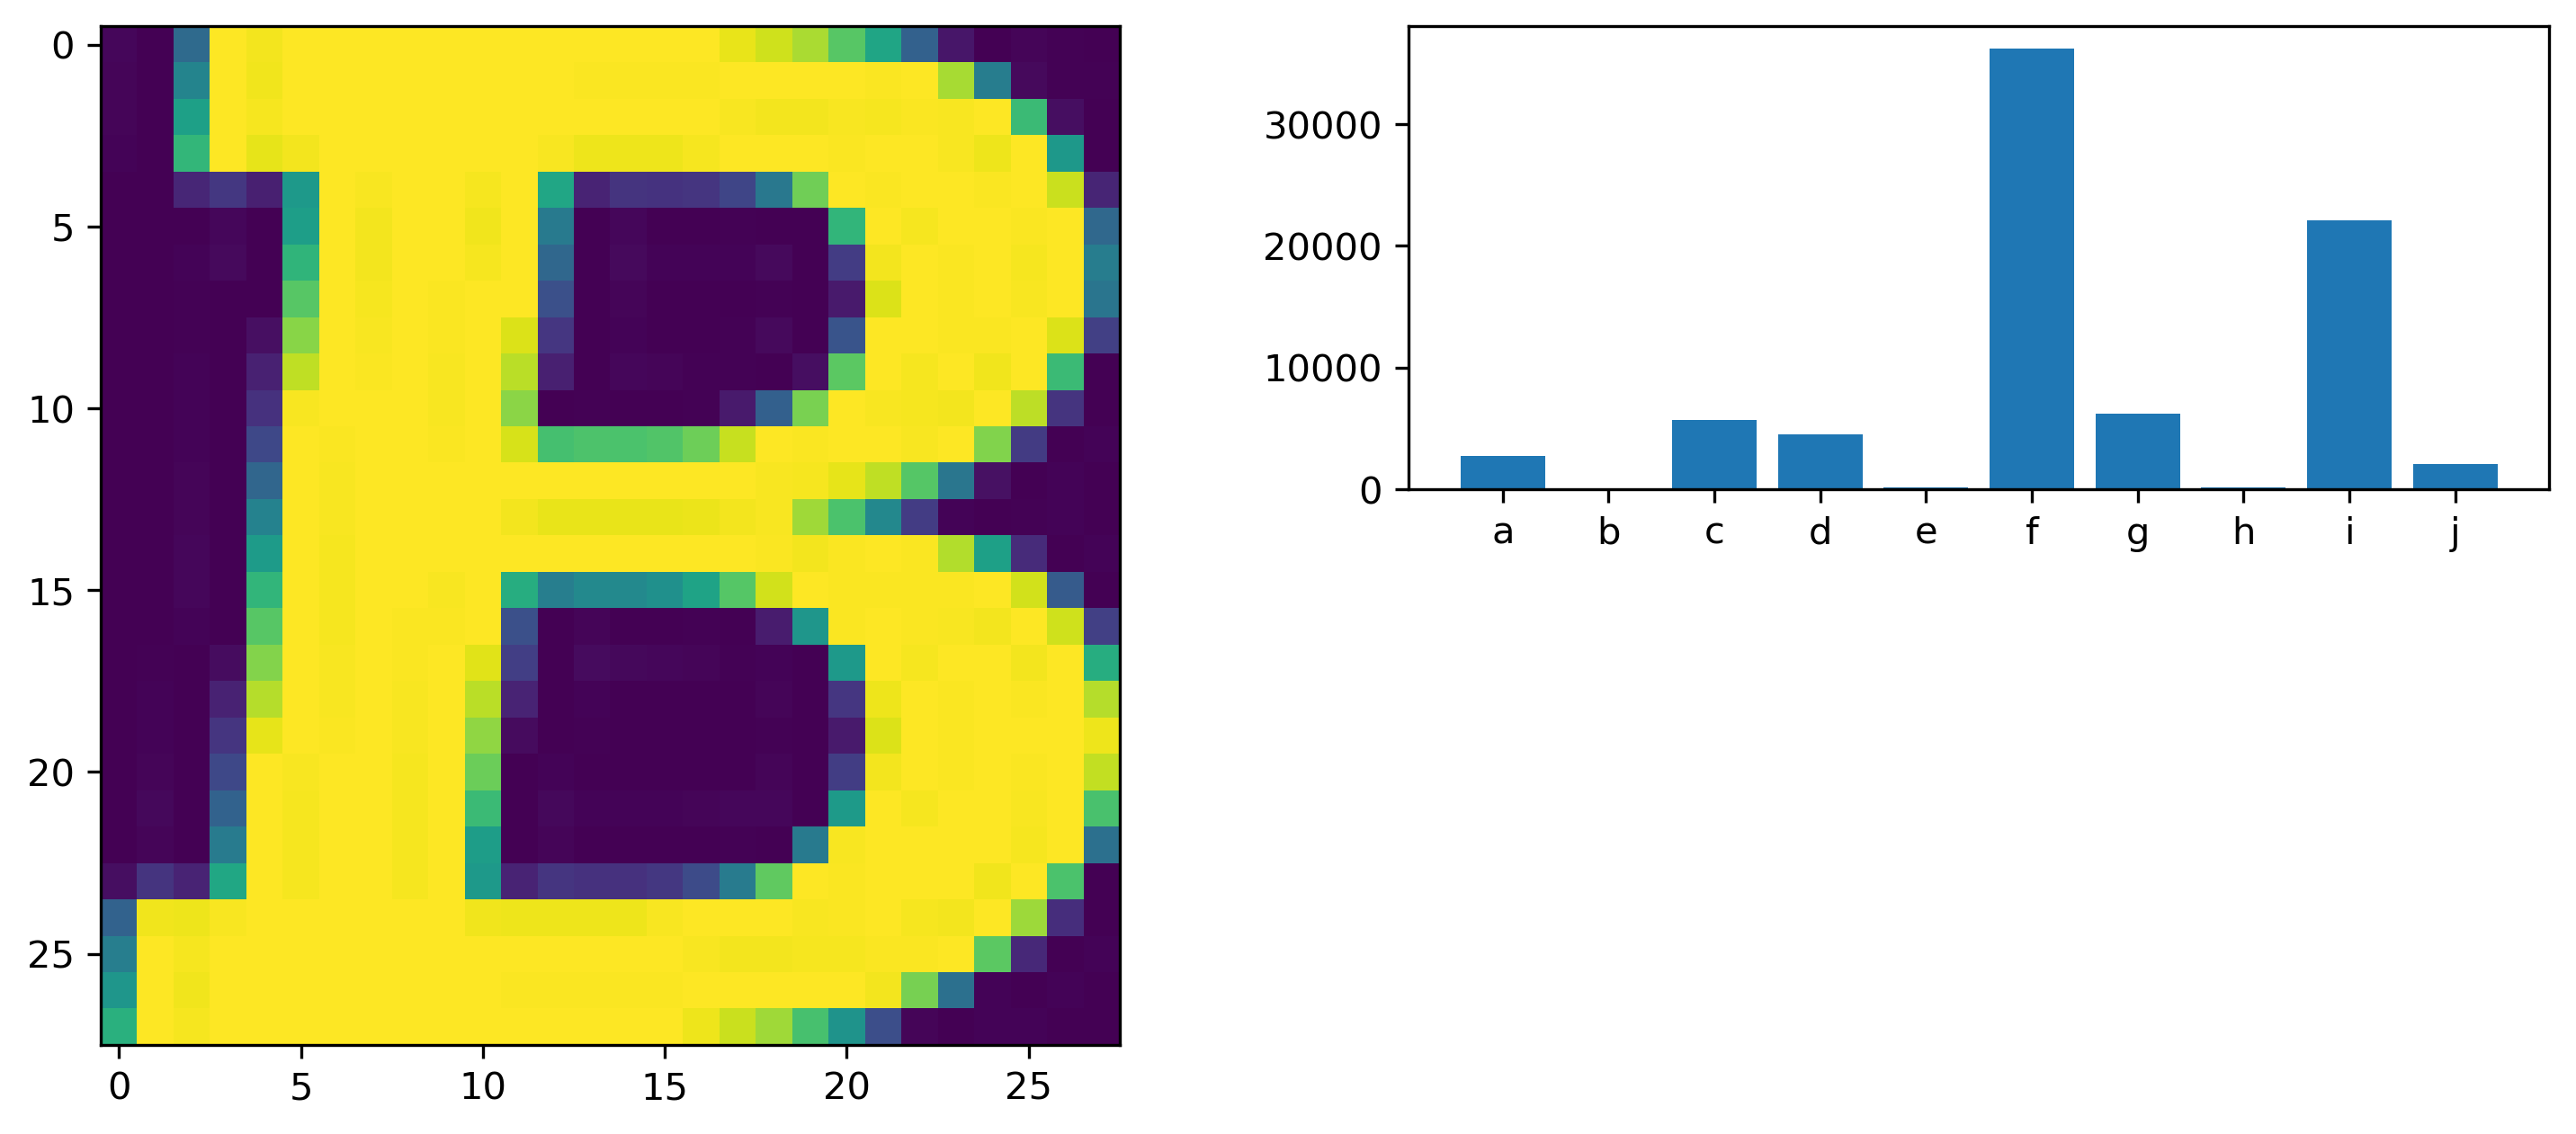
\includegraphics[width=.95\linewidth]{parts/Images/B.png}
  \caption{Uncertainty in out-of-distribution examples}
  \label{fig:B}
\end{subfigure}%
\begin{subfigure}{.5\textwidth}
  \centering
  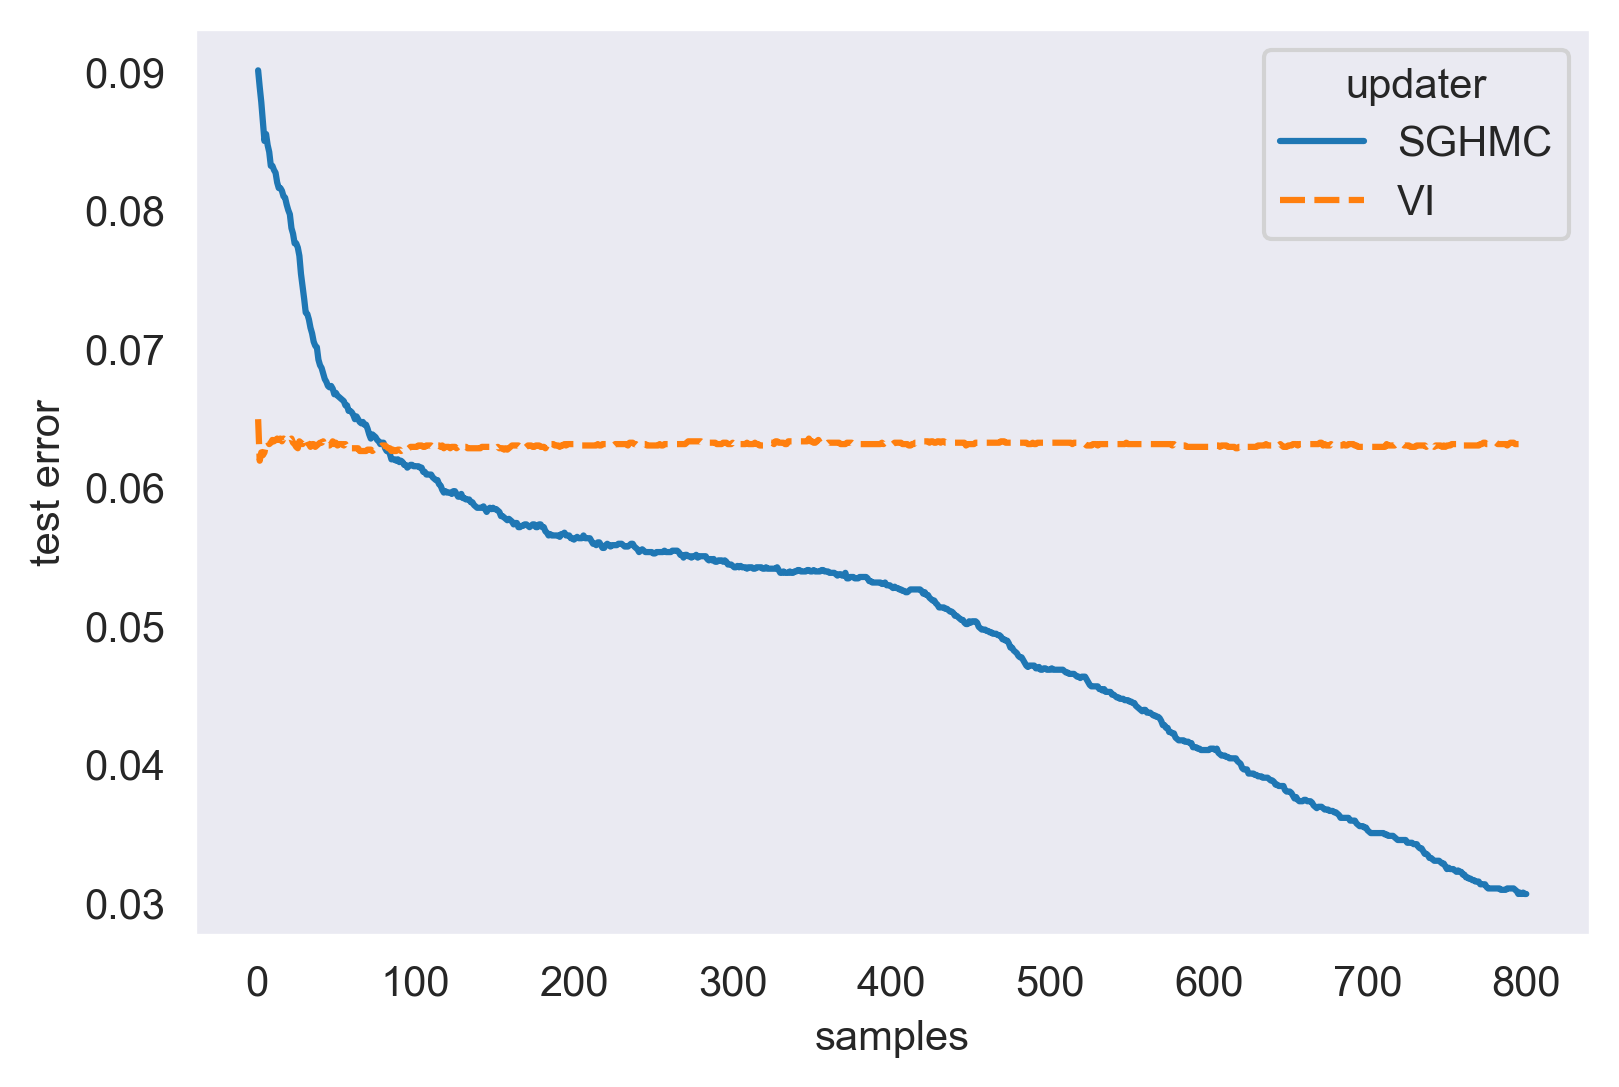
\includegraphics[width=.95\linewidth]{parts/Images/VI_SGHMC.png}
  \caption{VI and SGHMC on MNIST}
  \label{fig:VI}
\end{subfigure}
\caption{{\bf Left} (a) illustrates that we get uncertainty estimates on out-of-distribution examples. {\bf Right} (b) compares VI (Renyi ELBO, $\alpha = 0.01$, \texttt{num\_particles} $= 2$) and SGHMC ($\eta = 2.0\times 10^{-6}, \alpha=0.01, \texttt{resample\_n} =0$) on MNIST. For VI we draw 80000 samples from the variational posterior $q_{\phi}$ and report the test error by Bayesian averaging. For SGHMC we do the same, except we are approximately sampling from the true posterior $p(\theta \: | \mathcal{D} \:)$.}
\label{fig:demo}
\end{figure}
The initial results suggest that SGHMC performs better than VI in this setting, although this is not the full picture. Once VI fits the variational posterior distribution $q_{\phi}$ as closely as possible to the true posterior it takes only hundreds of samples to characterise $q_{\phi}$, whereas SGHMC requires several more samples to characterise the true posterior. In practice storing thousands of parameterisations of the same NN is very costly and so this is probably why VI is a more popular choice for Bayesian inference. 

We conclude this section by demonstrating our algorithms can be applied to other datasets and more complicated models, \cref{fig:fashionMNIST} presents the results of running the same BNN architecture on FashionMNIST, and \cref{fig:CIFAR10} demonstrates that our implementation of SGHMC can be used with convolutional neural networks (CNNs).
\begin{figure}[h!]
\centering
\begin{subfigure}{.5\textwidth}
  \centering
  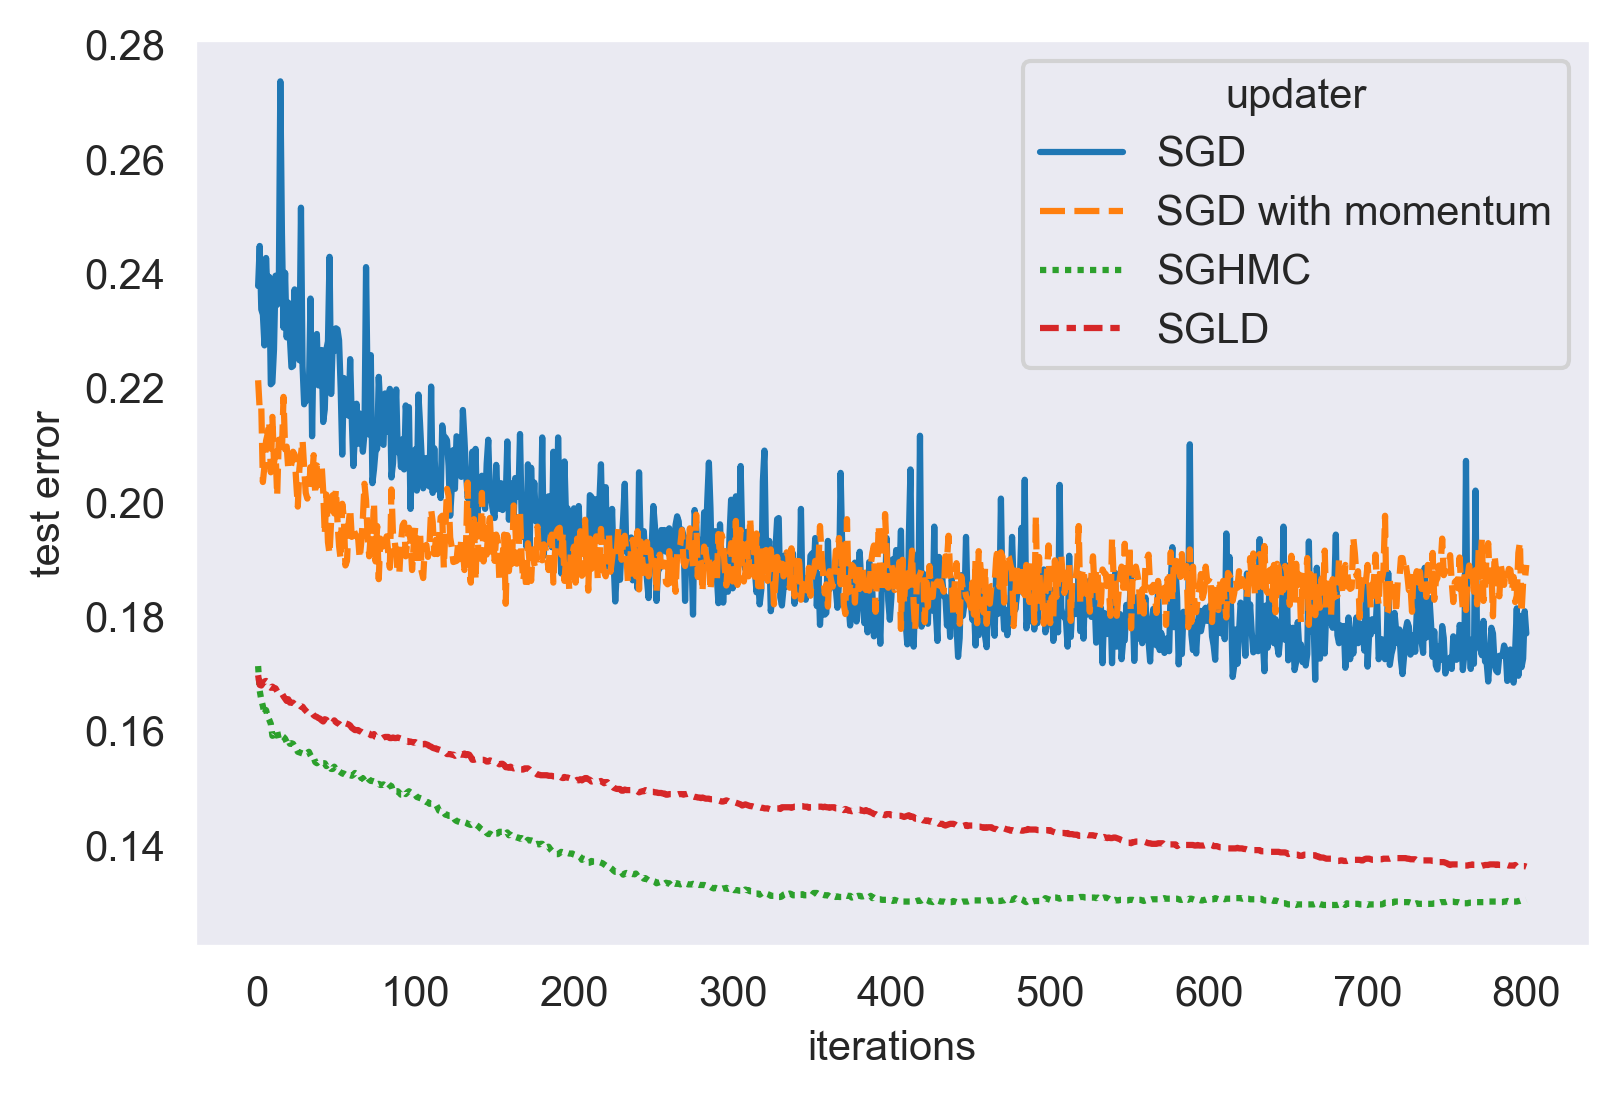
\includegraphics[width=.95\linewidth]{parts/Images/fashion-mnist.png}
  \caption{Experiment on FashionMNIST}
  \label{fig:fashionMNIST}
\end{subfigure}%
\begin{subfigure}{.5\textwidth}
  \centering
  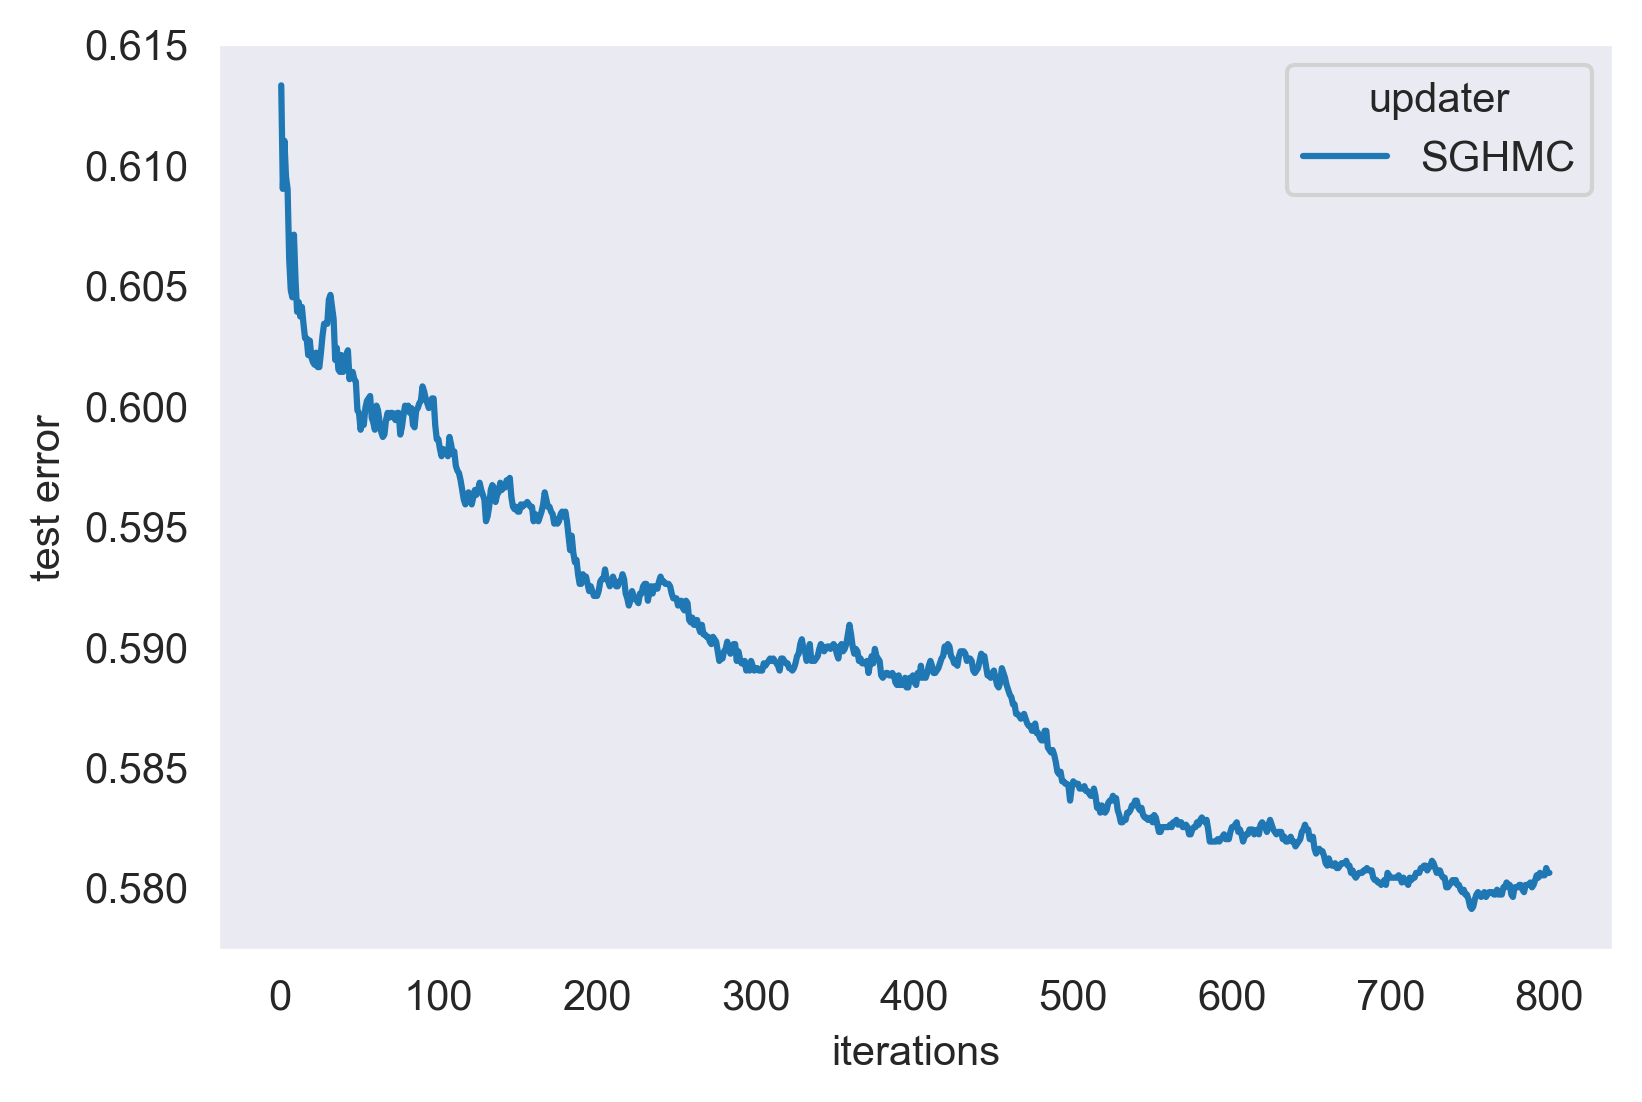
\includegraphics[width=.95\linewidth]{parts/Images/CIFAR10.png}
  \caption{Convolutional BNN on CIFAR10}
  \label{fig:CIFAR10}
\end{subfigure}
\caption{{\bf Left} (a) FashionMNIST classification; SGHMC ($\eta = 1.0\times 10^{-6}, \alpha=0.01, \texttt{resample\_n} =0$ ), SGLD ($\eta = 1.0\times 10^{-5}$), SGD ($\eta = 1.0\times 10^{-5}$), SGD with momentum ($\eta = 1.0\times 10^{-6}, \alpha=0.01$); \texttt{warmup\_epochs} $= 100$. {\bf Right} (b) Convolutional BNN with 2 convolutional layers, batch norm, max pooling and tanh activations followed by two Bayesian linear layers with tanh activation;  SGHMC ($\eta = 1.0\times 10^{-6}, \alpha=0.01, \texttt{resample\_n} =0$ ) ; \texttt{warmup\_epochs} $= 150$.}
\label{fig:other-datasets}
\end{figure}
\end{document}
